\section{Cache}



\subsubsection{Principle of Locality and Memory Hierarchy}

\begin{concept}{Memory Hierarchy and Locality}\\
Programs usually access small regions of memory in a given interval of time. \\
The memory hierarchy in computer systems is designed to exploit the principle of locality:
\begin{itemize}
    \item \textbf{Spatial Locality}: If a memory location is accessed, nearby locations are likely to be accessed soon
    \item $\rightarrow$ Current data location is likely being close to next accessed location
    \begin{itemize}
        \item Example: Sequential access to array elements
    \end{itemize}
    \item \textbf{Temporal Locality}: If a memory location is accessed, it's likely to be accessed again soon
    \item $\rightarrow$ Current data location is likely being accessed again in near future
    \begin{itemize}
        \item Example: Loop variables, frequently called functions
    \end{itemize}
\end{itemize}
The memory hierarchy takes advantage of these patterns:
\begin{itemize}
    \item Faster, smaller memories (cache) store recently/frequently accessed data
    \item Larger, slower memories (main memory, disk) store less frequently accessed data
\end{itemize}
\end{concept}

\begin{code}{Principle of Locality}
\begin{lstlisting}[language=C, style=basesmol]
for (int i = 0; i < N; i++) {   // incremental access
    a[i] = b[i];                // spatial locality
}

if (a[1234] == a[4321]) {       // temporal locality
    a[1234] = 0;                // access to same location again
} 
\end{lstlisting}  
\end{code}

\begin{definition}{Memory Hierarchy Levels}
Typical memory hierarchy in a modern system:
\begin{itemize}
    \item \textbf{CPU Registers}: Fastest, smallest (bytes)
    \item \textbf{L1 Cache}: Very fast, small (KB)
    \begin{itemize}
        \item Often split into instruction and data caches (Harvard architecture)
    \end{itemize}
    \item \textbf{L2 Cache}: Fast, medium size (hundreds of KB)
    \item \textbf{L3 Cache}: Moderately fast, larger (MB)
    \item \textbf{Main Memory (RAM)}: Slower, much larger (GB)
    \item \textbf{Secondary Storage}: Very slow, huge (TB)
\end{itemize}
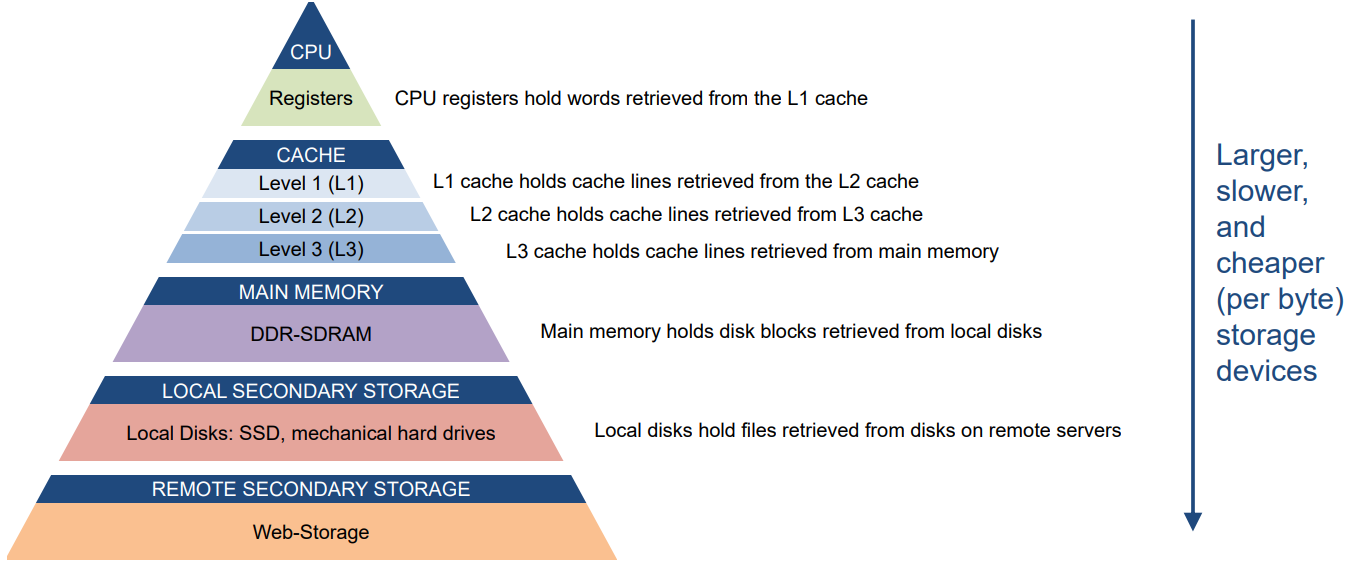
\includegraphics[width=\linewidth]{memory_hierarchy_levels.png}
\end{definition}

\begin{remark}
    \textbf{Situation:}
    \begin{itemize}
        \item Processor: fast cycle time
        \item Fast DRAM: Single accesses have large overhead (slow), efficiently reads only in bursts
        \item $\rightarrow$ bridging the gap such that pipelining and the bursts are effective!
    \end{itemize}
\textbf{Goal:}
\begin{itemize}
    \item Access 'slower' main memory in bursts and maintain a fast cache memory for fast single accesses
    \item But: Data consistency must be carefully managed, such that both, cache and main memory have the same data
\end{itemize}
\end{remark}

\subsection{Cache Mechanics}

\begin{definition}{Cache Levels} Typical Cache Architecture\\
    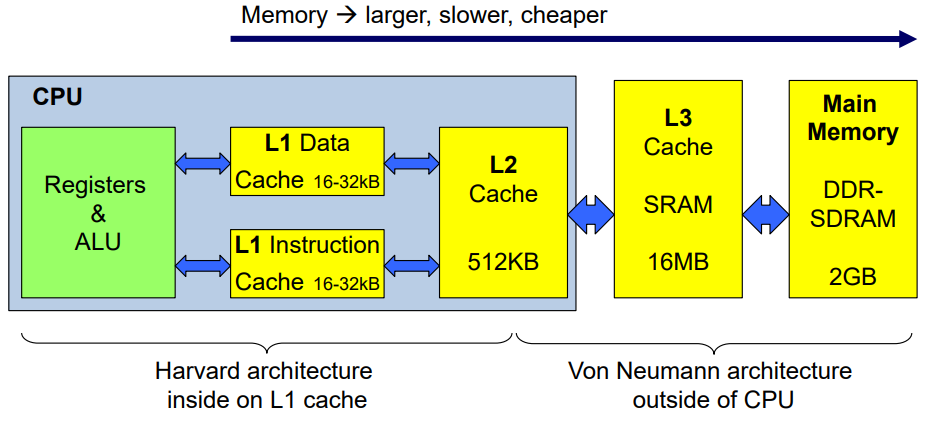
\includegraphics[width=\linewidth]{cache_architecture.png}    
\end{definition}

\begin{concept}{Cache Operation}\\
A cache is a small, fast memory that stores copies of data from frequently used main memory locations:
\begin{itemize}
    \item Main memory is divided into fixed-size blocks
    \item Cache holds copies of some memory blocks
    \item When CPU needs data:
    \begin{itemize}
        \item \textbf{Cache Hit}: Data is in cache $\rightarrow$ fast access
        \item \textbf{Cache Miss}: Data not in cache $\rightarrow$ fetched from main memory, then stored in cache for future access
    \end{itemize}
\end{itemize}
\end{concept}

\begin{definition}{Cache Terminology}\\
Key terms in cache design:
\begin{itemize}
    \item \textbf{Cache Line}: Basic unit of data transfer (typically 32-128 bytes)
    \item \textbf{Tag}: Part of address that identifies which memory block is stored
    \item \textbf{Valid Bit}: Indicates if the cache line contains valid data
    \item \textbf{Hit Rate}: Percentage of memory accesses found in cache
    \item \textbf{Miss Rate}: Percentage of memory accesses not found in cache
    \item \textbf{Hit Time}: Time to access data in cache
    \item \textbf{Miss Penalty}: Extra time required to fetch data from main memory
\end{itemize}
\end{definition}

\raggedcolumns
\columnbreak

\subsection{Cache Organization}

\mult{2}

\begin{definition}{Memory Addressing for Cache}\\
A memory address is typically divided into:
\begin{itemize}
    \item \textbf{Tag}: Identifies which memory block is stored
    \item \textbf{Index}: Determines location in cache (for direct-mapped and set-associative)
    \item \textbf{Offset}: Identifies specific byte within the block
\end{itemize}
\begin{center}
\begin{tabular}{|c|c|c|}
\hline
Tag & Index & Offset \\
\hline
\end{tabular}
\end{center}
The size of each field depends on the cache organization.
\end{definition}

\begin{concept}{Fully Associative Cache}\\
    Any memory block can be stored in any cache line
\begin{itemize}
    \item Address format: [Tag | Offset]
    \item Each cache line stores:
    \begin{itemize}
        \item Valid bit (is data valid?)
        \item Tag (which memory block)
        \item Data (contents of memory block)
    \end{itemize}
    \item On memory access, the tag is compared with all cache lines in parallel
    \item Highest flexibility, best hit rate
    \item Requires many comparators (one per cache line)
    \item Complex hardware: requires comparing tag with all cache lines
\end{itemize}
\end{concept}

\begin{concept}{Direct Mapped Cache}\\
    Each memory block maps to exactly one cache line
\begin{itemize}
    \item Mapping function: $\text{Line} = \text{Block} \bmod m$ (where $m$ is number of cache lines)
    \item Address format: [Tag | Index | Offset]
    \item The index directly selects which cache line to check
    \item Only one tag comparison needed
    \item Simple hardware but can suffer from conflict misses (resulting in lower hit rate)
    \begin{itemize}
        \item Different memory blocks mapping to the same cache line
    \end{itemize}
\end{itemize}
\end{concept}

\begin{concept}{N-Way Set Associative Cache}\\
    Cache is divided into sets, each containing N lines
\begin{itemize}
    \item Memory block maps to a specific set, can go in any line within that set
    \item Mapping function: $\text{Set} = \text{Block} \bmod s$ (where $s$ is number of sets)
    \item Address format: [Tag | Set Index | Offset]
    \item Set index selects which set to check
    \item N tag comparisons needed (one per line in set)
    \item Compromise between fully associative and direct mapped 
    \begin{itemize}
        \item More flexible than direct mapped
        \item Less hardware than fully associative
    \end{itemize}
\end{itemize}
\end{concept}

\multend 

\subsubsection{Cache Organization and Addressing}

\begin{KR}{Analyzing Cache Organization}
\paragraph{Identify cache parameters}
\begin{itemize}
    \item Cache size: Total data storage capacity
    \item Block/line size: Size of each cache line (typically 16-128 bytes)
    \item Associativity: Number of ways (n=1 for direct mapped, n=cache size/block size for fully associative)
    \item Number of sets: s = cache size / (block size × associativity)
\end{itemize}

\paragraph{Address decomposition}
\begin{itemize}
    \item Divide address into tag, index, and offset fields
    \item Offset bits = log$_2$(block size)
    \item Index bits = log$_2$(number of sets)
    \item Tag bits = address bits - (offset bits + index bits)
\end{itemize}

\paragraph{Determine cache organization}
\begin{itemize}
    \item \textbf{Direct mapped cache:}
    \begin{itemize}
        \item One line per set (associativity = 1)
        \item Number of sets = cache size / block size
        \item Index field directly selects the cache line
    \end{itemize}
    \item \textbf{Fully associative cache:}
    \begin{itemize}
        \item One set with all lines (number of sets = 1)
        \item No index field, only tag and offset
        \item Requires comparison with all cache line tags
    \end{itemize}
    \item \textbf{N-way set associative cache:}
    \begin{itemize}
        \item N lines per set
        \item Number of sets = cache size / (N × block size)
        \item Index field selects the set, tag comparison within the set
    \end{itemize}
\end{itemize}

\paragraph{Map memory addresses to cache}
\begin{itemize}
    \item Calculate set number: (address / block size) mod (number of sets)
    \item Calculate tag: address / (block size × number of sets)
    \item Calculate offset: address mod block size
\end{itemize}
\end{KR}

\begin{example2}{Cache Organization Analysis}\\
Consider a system with a 4 KiB direct-mapped cache with 16-byte cache lines. The system uses 32-bit byte addresses.

\begin{enumerate}
    \item How many cache lines are there?
    \item How many bits are needed for the tag, index, and offset?
    \item For memory address 0x1234ABCD, determine the tag, index, and offset.
    \item Which other addresses would map to the same cache line?
\end{enumerate}

\tcblower

1. \textbf{Number of cache lines:}
   \begin{itemize}
     \item Cache size = 4 KiB = 4096 bytes
     \item Line size = 16 bytes
     \item Number of lines = 4096 / 16 = 256 lines
   \end{itemize}

2. \textbf{Address bit fields:}
   \begin{itemize}
     \item Offset bits = log$_2$(16) = 4 bits (addresses byte within the line)
     \item Index bits = log$_2$(256) = 8 bits (selects the cache line)
     \item Tag bits = 32 - (4 + 8) = 20 bits (identifies which memory block is cached)
   \end{itemize}

3. \textbf{Address decomposition for 0x1234ABCD:}
   \begin{itemize}
     \item Convert to binary: 0001 0010 0011 0100 1010 1011 1100 1101
     \item Offset: last 4 bits = 1101 = 0xD
     \item Index: next 8 bits = 1011 1100 = 0xBC
     \item Tag: remaining 20 bits = 0001 0010 0011 0100 1010 = 0x1234A
   \end{itemize}

4. \textbf{Other addresses mapping to the same cache line:}
   \begin{itemize}
     \item Addresses with the same index (0xBC) but different tags would map to the same line
     \item General form: 0xXXXXXBCY where:
     \begin{itemize}
       \item XXXXX can be any value except 0x1234A (different tag)
       \item BC is fixed (same index)
       \item Y can be any value from 0 to F (different offset within the line)
     \end{itemize}
     \item Examples: 0x0034ABCD, 0x5678ABCF, 0x9ABCDBCE, etc.
     \item These addresses would cause cache conflicts if accessed in sequence
   \end{itemize}
\end{example2}

\begin{example2}{Cache Organization Calculation}\\
For a 16KB cache with 64-byte lines, calculate address breakdown for:
\begin{itemize}
\item Direct mapped
\item 4-way set associative
\end{itemize}
\tcblower
Given:
\begin{itemize}
    \item Cache size = 16KB = 16,384 bytes
    \item Line size = 64 bytes
\end{itemize}

1. Direct Mapped Cache:
\begin{itemize}
    \item Number of cache lines = Cache size / Line size = 16,384 / 64 = 256 lines
    \item Index bits = $\log_2(256)$ = 8 bits
    \item Offset bits = $\log_2(64)$ = 6 bits
    \item For 32-bit address: Tag = 32 - 8 - 6 = 18 bits
\end{itemize}
Address format: [18-bit Tag | 8-bit Index | 6-bit Offset]
\vspace{2mm}\\
2. 4-Way Set Associative:
\begin{itemize}
    \item Number of sets = Cache size / (Line size × Associativity) = 16,384 / (64 × 4) = 64 sets
    \item Set index bits = $\log_2(64)$ = 6 bits
    \item Offset bits = $\log_2(64)$ = 6 bits
    \item For 32-bit address: Tag = 32 - 6 - 6 = 20 bits
\end{itemize}   
Address format: [20-bit Tag | 6-bit Set Index | 6-bit Offset]
\end{example2}

\subsection{Cache Performance}

\begin{definition}{Cache Miss Types}
Three fundamental types of cache misses:
\begin{itemize}
    \item \textbf{Compulsory Misses} (Cold Misses):
    \begin{itemize}
        \item First access to a block, must be fetched from memory
        \item Unavoidable, regardless of cache size or organization
    \end{itemize}
    \item \textbf{Capacity Misses}:
    \begin{itemize}
        \item Cache too small to hold all blocks needed during program execution
        \item Blocks evicted and later needed again
        \item Can be reduced by increasing cache size
    \end{itemize}
    \item \textbf{Conflict Misses}:
    \begin{itemize}
        \item Multiple blocks map to same cache line/set
        \item More common in direct mapped, less in set associative
        \item Can be reduced by increasing associativity
    \end{itemize}
\end{itemize}
\end{definition}

\begin{formula}{Cache Performance}\\
Average memory access time (AMAT) can be calculated as:
$$
AMAT = \text{Hit Time} + \text{Miss Rate} \times \text{Miss Penalty}
$$

Example:
\begin{itemize}
    \item Hit Time = 1 cycle
    \item Miss Penalty = 100 cycles
    \item Miss Rate = 3\% (0.03)
\end{itemize}
$$
AMAT = 1 + 0.03 \times 100 = 1 + 3 = 4 \text{ cycles}
$$

Reducing miss rate from 3\% to 1\% changes AMAT to:
$$
AMAT = 1 + 0.01 \times 100 = 1 + 1 = 2 \text{ cycles}
$$
This is a 50\% performance improvement!
\end{formula}

\begin{concept}{Cache Size vs. Hit Rate}\\
Relationship between cache parameters and hit rate:
\begin{itemize}
    \item Increasing cache size improves hit rate
    \begin{itemize}
        \item But with diminishing returns
        \item Larger cache may have longer hit time
    \end{itemize}
    \item Increasing associativity improves hit rate
    \begin{itemize}
        \item Greatest benefit from direct-mapped to 2-way
        \item Diminishing returns beyond 4-way or 8-way
        \item Higher associativity increases complexity and hit time
    \end{itemize}
    \item Increasing block size improves spatial locality exploitation
    \begin{itemize}
        \item But increases miss penalty
        \item Very large blocks may cause pollution
    \end{itemize}
\end{itemize}
\end{concept}

\subsection{Cache Performance Analysis}

\begin{KR}{Analyzing Cache Hit Rates and Performance}
\paragraph{Calculate basic cache metrics}
\begin{itemize}
    \item Hit rate = Number of hits / Total number of accesses
    \item Miss rate = 1 - Hit rate
    \item Average memory access time (AMAT) = Hit time + (Miss rate × Miss penalty)
\end{itemize}

\paragraph{Identify types of cache misses}
\begin{itemize}
    \item \textbf{Compulsory misses:} First access to a block (cold start)
    \item \textbf{Capacity misses:} Cache is full, blocks need to be evicted
    \item \textbf{Conflict misses:} In direct-mapped or set-associative caches when multiple blocks map to same set
\end{itemize}

\paragraph{Analyze memory access patterns}
\begin{itemize}
    \item Spatial locality: Sequential or nearby accesses
    \item Temporal locality: Repeated accesses to same location
    \item Stride patterns: Regular jumps between memory locations
\end{itemize}

\paragraph{Evaluate impact of cache parameters}
\begin{itemize}
    \item Effect of cache size: Larger cache reduces capacity misses
    \item Effect of block size: Larger blocks improve spatial locality, but may increase miss penalty
    \item Effect of associativity: Higher associativity reduces conflict misses
    \item Effect of replacement policy: LRU, FIFO, Random - impact on hit rate
\end{itemize}
\end{KR}

\begin{example2}{Cache Performance Calculation}\\
Consider a system with the following cache parameters:
\begin{itemize}
    \item Cache access time: 1 processor cycle
    \item Main memory access time: 100 processor cycles
    \item Miss rate for cache configuration A: 3\%
    \item Miss rate for cache configuration B: 1\%
\end{itemize}

\begin{enumerate}
    \item Calculate the average memory access time (AMAT) for both configurations
    \item If configuration B has twice the associativity of A, explain why the miss rate improved
    \item If the program executes 1 million memory accesses, how many cycles are saved by using configuration B instead of A?
\end{enumerate}

\tcblower

1. \textbf{Calculate AMAT for both configurations:}
   \begin{itemize}
     \item AMAT = Hit time + (Miss rate × Miss penalty)
     \item For configuration A:
     \begin{itemize}
       \item AMAT$_A$ = 1 cycle + (0.03 × 100 cycles) = 1 + 3 = 4 cycles
     \end{itemize}
     \item For configuration B:
     \begin{itemize}
       \item AMAT$_B$ = 1 cycle + (0.01 × 100 cycles) = 1 + 1 = 2 cycles
     \end{itemize}
   \end{itemize}

2. \textbf{Effect of increased associativity:}
   \begin{itemize}
     \item Higher associativity reduces conflict misses
     \item In configuration A (lower associativity), more memory blocks map to the same cache set
     \item With configuration B (doubled associativity), each set can hold twice as many blocks
     \item This reduces the chance of having to evict a useful block due to set conflicts
     \item The improved miss rate (from 3\% to 1\%) is primarily due to the reduction in conflict misses
     \item Note that capacity misses and compulsory misses would remain the same
   \end{itemize}

3. \textbf{Cycles saved:}
   \begin{itemize}
     \item Total accesses = 1,000,000
     \item Cycles for configuration A = 1,000,000 × 4 = 4,000,000 cycles
     \item Cycles for configuration B = 1,000,000 × 2 = 2,000,000 cycles
     \item Cycles saved = 4,000,000 - 2,000,000 = 2,000,000 cycles
   \end{itemize}

Therefore, using configuration B saves 2 million processor cycles for the program, cutting the memory access time in half.
\end{example2}

\subsection{Replacement and Write Strategies}

\mult{2}

\begin{definition}{Replacement Strategies}\\
When a new block must be loaded into a full cache set, a replacement strategy determines which existing block to evict:
\begin{itemize}
    \item \textbf{Least Recently Used (LRU)}:
    \begin{itemize}
        \item Evict the block that hasn't been accessed for the longest time
        \item Good performance but complex to implement for high associativity
    \end{itemize}
    \item \textbf{Least Frequently Used (LFU)}:
    \begin{itemize}
        \item Evict the block that has been accessed least often
        \item Requires access counters for each block
    \end{itemize}
    \item \textbf{First-In First-Out (FIFO)}:
    \begin{itemize}
        \item Evict the block that has been in cache longest
        \item Simpler to implement than LRU
    \end{itemize}
    \item \textbf{Random}:
    \begin{itemize}
        \item Evict a random block
        \item Simplest to implement
        \item Performance often surprisingly close to LRU
    \end{itemize}
\end{itemize}
\end{definition}

\begin{definition}{Write Strategies}\\
When a write operation hits in cache, two main strategies exist:
\begin{itemize}
    \item \textbf{Write-Through}:
    \begin{itemize}
        \item Write data to both cache and main memory
        \item Memory always consistent with cache
        \item Slower for writes (must wait for memory)
        \item Simpler coherence in multiprocessor systems
    \end{itemize}
    \item \textbf{Write-Back}:
    \begin{itemize}
        \item Write data only to cache
        \item Mark block as "dirty"
        \item Write to memory only when block is evicted
        \item Faster for repeated writes to same block
        \item More complex coherence handling
    \end{itemize}
\end{itemize}

For write misses, two approaches:
\begin{itemize}
    \item \textbf{Write-Allocate}:
    \begin{itemize}
        \item Fetch block into cache, then update
        \item Works well with write-back
    \end{itemize}
    \item \textbf{No-Write-Allocate}:
    \begin{itemize}
        \item Write directly to memory, don't fetch block
        \item Works well with write-through
    \end{itemize}
\end{itemize}
\end{definition}

\multend

\subsection{Programmer's Perspective}

\begin{concept}{Cache Performance Optimization}\\
General guidelines for cache-friendly programming:
\begin{itemize}
    \item \textbf{Loop Interchange}: Reorder nested loops to access memory sequentially
    \item \textbf{Loop Blocking/Tiling}: Break large loops into smaller chunks that fit in cache
    \item \textbf{Data Alignment}: Align data structures to cache line boundaries
    \item \textbf{Structure Packing}: Organize structure fields to minimize cache line usage
    \item \textbf{Prefetching}: Load data into cache before it's needed
    \item \textbf{Reduce Working Set Size}: Keep active data small enough to fit in cache
\end{itemize}
\end{concept}


\begin{theorem}{Optimizing Code for Cache Performance}
\paragraph{Analyze array access patterns}
\begin{itemize}
    \item Understand memory layout in your language (e.g., row-major in C, column-major in Fortran)
    \item Match loop iteration order to memory layout (e.g., for C: outer loop for rows, inner loop for columns)
    \item Avoid strided access patterns that lead to frequent cache misses
\end{itemize}

\paragraph{Improve spatial locality}
\begin{itemize}
    \item Place related data together in memory
    \item Use structures instead of separate arrays for related data
    \item Pad data structures to align with cache lines when appropriate
\end{itemize}

\paragraph{Improve temporal locality}
\begin{itemize}
    \item Reuse data while it's still in cache
    \item Use blocking/tiling for matrix operations to maximize data reuse
    \item Process data in chunks that fit in cache
\end{itemize}

\paragraph{Avoid cache conflicts}
\begin{itemize}
    \item Be aware of array sizes that are powers of 2, which can lead to systematic conflicts
    \item Pad arrays to avoid conflict misses in direct-mapped or set-associative caches
    \item Consider memory alignment to reduce conflicts
\end{itemize}
\end{theorem}

\begin{KR}{Cache-Friendly Programming}

\textbf{Maximize spatial locality}:
Access memory in sequential patterns whenever possible.

\textbf{Maximize temporal locality}:
Reuse recently accessed data before it gets evicted from cache.

\textbf{Be aware of cache line size}:
Structure data to minimize cache line crossings.

\textbf{Consider memory layout}:
Organize multidimensional arrays to match access patterns.

\begin{lstlisting}[language=C, style=basesmol]
// Cache-unfriendly code (column-major traversal of row-major array)
for (j = 0; j < N; j++) {
    for (i = 0; i < N; i++) {
        sum += array[i][j];  // Poor spatial locality
    }
}
// Cache-friendly code (row-major traversal of row-major array)
for (i = 0; i < N; i++) {
    for (j = 0; j < N; j++) {
        sum += array[i][j];  // Good spatial locality
    }
}
\end{lstlisting}
\end{KR}


\begin{example}
Consider a matrix multiplication function for 1000×1000 matrices. Two implementations are shown:

\begin{lstlisting}[language=C, style=basesmol]
// Version A - Row by Column
for(i = 0; i < 1000; i++) {
    for(j = 0; j < 1000; j++) {
        for(k = 0; k < 1000; k++) {
            C[i][j] += A[i][k] * B[k][j];
        }
    }
}
// Version B - Blocked/Tiled
for(i = 0; i < 1000; i += 64) {
    for(j = 0; j < 1000; j += 64) {
        for(k = 0; k < 1000; k += 64) {
            for(ii = i; ii < min(i+64, 1000); ii++) {
                for(jj = j; jj < min(j+64, 1000); jj++) {
                    for(kk = k; kk < min(k+64, 1000); kk++) {
                        C[ii][jj] += A[ii][kk] * B[kk][jj];
                    }
                }
            }
        }
    }
}
\end{lstlisting}

Explain which version would perform better and why from a cache perspective.

\tcblower

Version B (the blocked/tiled implementation) will perform significantly better for the following cache-related reasons:

1. \textbf{Better spatial locality:}
   \begin{itemize}
     \item Version A accesses matrix B in column-major order (B[k][j]), which is inefficient in C where arrays are stored in row-major order
     \item This means adjacent accesses to B[k][j] jump by 1000 elements (entire row), causing frequent cache misses
     \item Version B limits this effect by working on small blocks at a time
   \end{itemize}

2. \textbf{Better temporal locality:}
   \begin{itemize}
     \item Version A loads each element of A and B 1000 times
     \item Version B loads each element only once within each block, then reuses it multiple times
     \item The blocks are sized (64×64) to fit within the cache, increasing reuse before eviction
   \end{itemize}

3. \textbf{Reduced cache pressure:}
   \begin{itemize}
     \item Version A works with the entire matrices at once
     \item Version B only needs to keep 3 blocks (A, B, C) in cache at a time
     \item For a typical L1 cache (32-64 KiB), the 64×64 blocks (32 KiB at 8 bytes per element) fit much better than the full matrices
   \end{itemize}

4. \textbf{Fewer cache misses:}
   \begin{itemize}
     \item Version A would cause frequent capacity misses as elements are evicted before reuse
     \item Version B significantly reduces capacity misses by ensuring blocks fit in cache
     \item Version B also reduces conflict misses by working with smaller, better aligned chunks
   \end{itemize}

This tiling technique is a classic cache optimization that can improve performance by orders of magnitude for matrix operations on large matrices.
\end{example}